\chapter{Simetría y grupos puntuales}\label{ch:b3:point-groups}

Si se gira un copo de nieve sesenta grados, nada cambia; si se gira una molécula de benceno
el mismo ángulo, sus seis carbonos y sus seis hidrógenos caen
exactamente en los lugares de los demás. La simetría de una molécula decide varias
de sus propiedades antes de cualquier cálculo: si puede tener momento
dipolar, si puede existir en dos formas que son imágenes especulares, cuáles de sus
vibraciones absorben luz infrarroja, qué orbitales pueden mezclarse. Para usarla, los químicos
tomaron de las matemáticas el lenguaje de los grupos. Este capítulo define las
\omterm{def:b3:point-groups:operation}{operaciones de simetría} de una molécula, las reúne en su \omterm{def:b3:point-groups:point-group}{grupo puntual},
da un procedimiento para encontrar ese grupo, demuestra dos teoremas sobre la polaridad y la
quiralidad, e introduce las \omterm{def:b3:point-groups:irrep}{tablas de caracteres} sobre las que se construye el
\cref{ch:b3:group-theory-applied}.

\begin{recall}
El volumen del primer año predijo las formas moleculares con el modelo RPECV, definió
el momento dipolar de una molécula polar y definió la quiralidad: una molécula
quiral no es superponible con su imagen especular. El volumen del segundo año usó
la simetría, en palabras, para construir los orbitales de fragmento de \ce{H2O} y \ce{NH3}.
\end{recall}

\begin{omfigure}
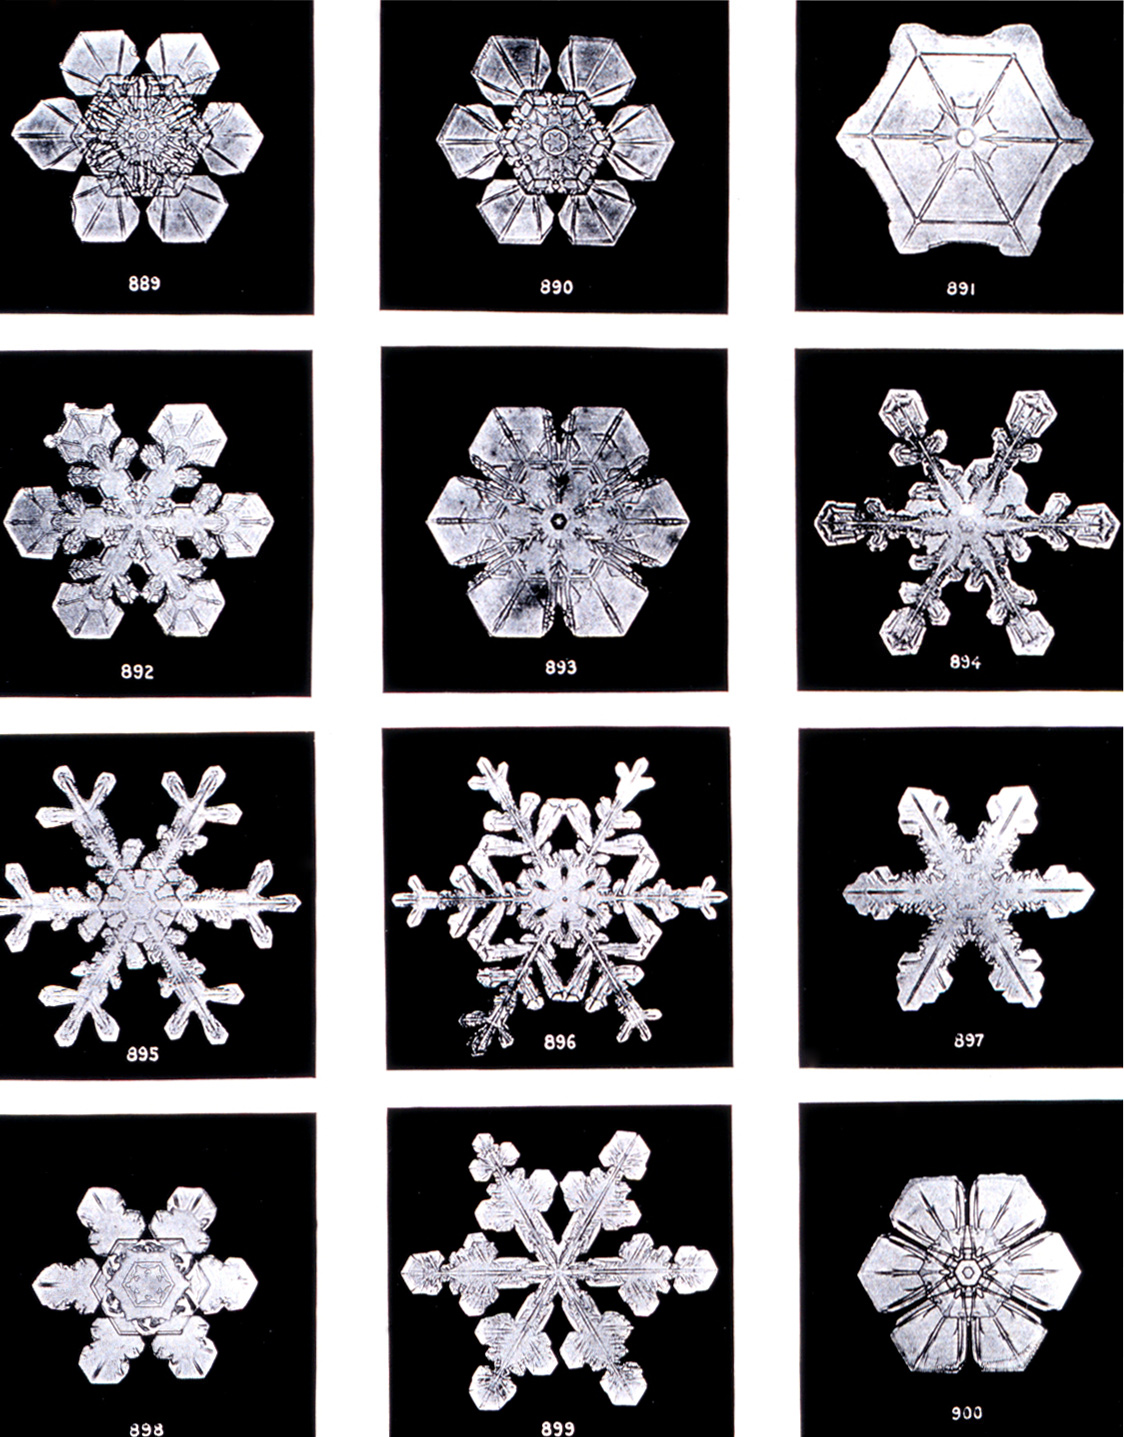
\includegraphics[width=0.4\linewidth]{images/book4/bentley-snowflakes.jpg}\hspace{1em}%
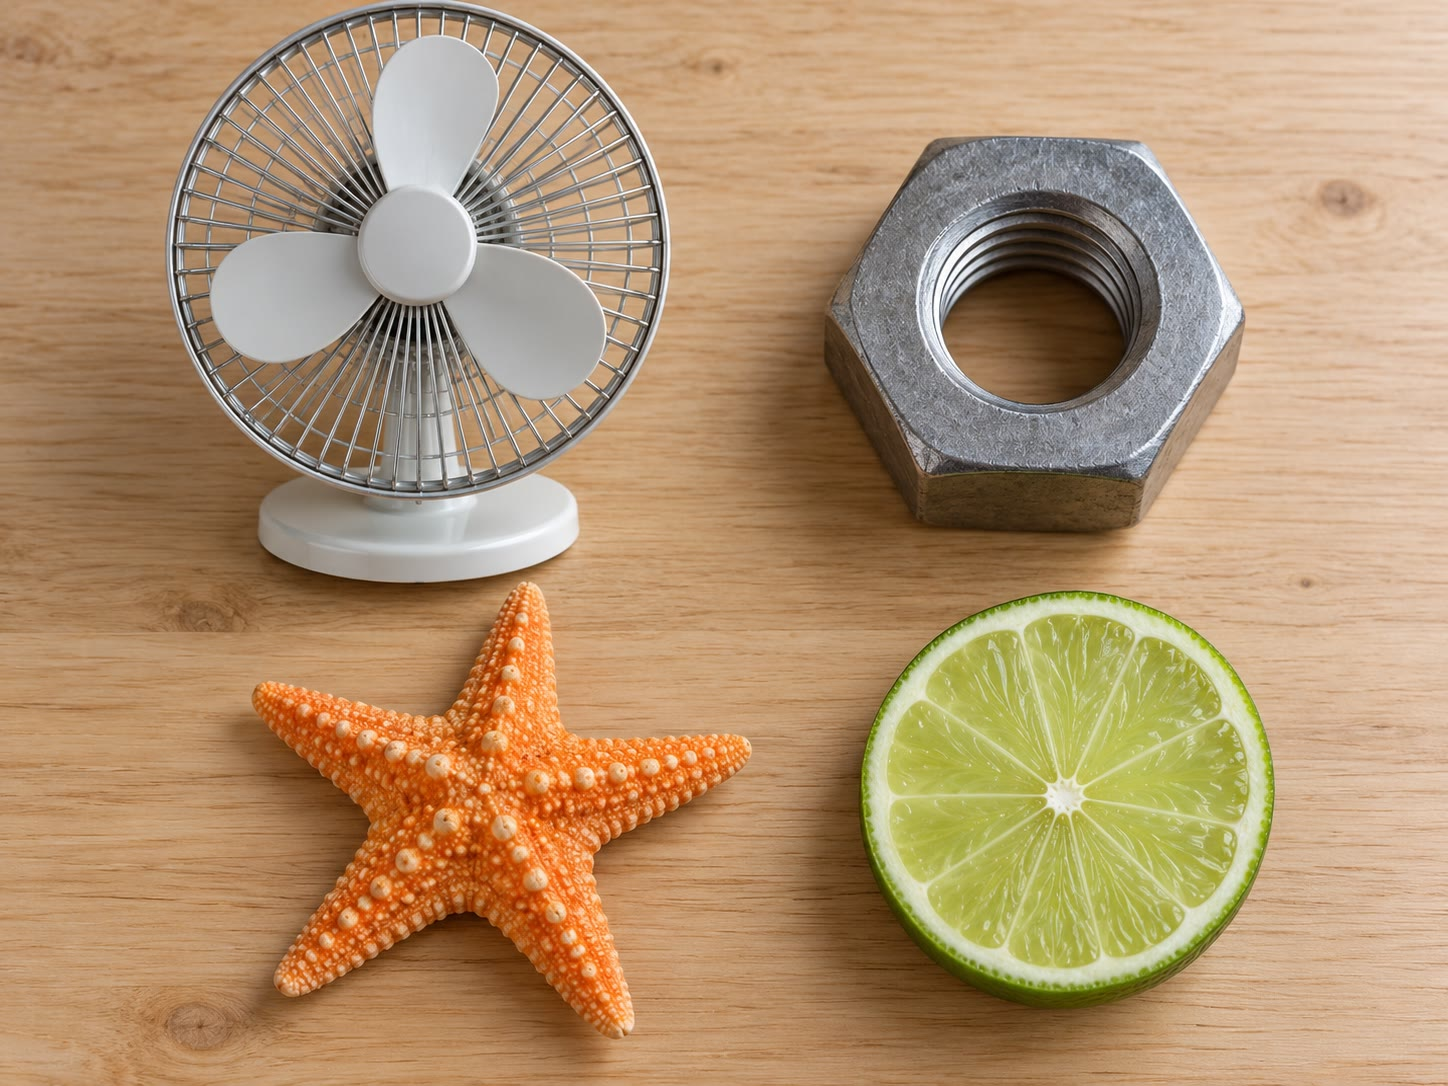
\includegraphics[width=0.48\linewidth]{images/book4/ai/b3-04-symmetric-objects.jpg}

{\small Izquierda: cristales de nieve fotografiados por Wilson Bentley hacia 1902,
cada uno con simetría de orden seis. Derecha: objetos cotidianos con simetría de rotación
de orden tres, seis y cinco.}
\end{omfigure}

\section{Operaciones y elementos de simetría}

\begin{definition}[Operación de simetría, elemento de simetría]\label{def:b3:point-groups:operation}
Una \emph{operación de simetría}\index{operacion de simetria@operación de simetría} es un movimiento o una
reflexión que deja una molécula en una configuración indistinguible de
la original (cada átomo en una posición ocupada antes por un átomo de la misma
clase). Un \emph{elemento de simetría}\index{elemento de simetria@elemento de simetría} es el objeto
geométrico ---un punto, una recta, un plano--- respecto del cual se efectúa
la operación.
\end{definition}

Toda molécula tiene la operación identidad $E$, que no hace nada. Las
demás son de cuatro tipos.

\begin{definition}[Eje de rotación propio, eje principal]\label{def:b3:point-groups:rotation}
Un \emph{eje de rotación propio}\index{eje de rotacion propio@eje de rotación propio} $C_n$ es una recta
en torno a la cual una rotación de $2\pi/n$ es una \omterm{def:b3:point-groups:operation}{operación de simetría}, que también se escribe
$C_n$; sus potencias $C_n^k$ son rotaciones de $2\pi k/n$, y $C_n^n = E$. El
eje de mayor $n$ es el \emph{eje principal}\index{eje principal}, que se toma
como $z$.
\end{definition}

\begin{definition}[Planos de simetría]\label{def:b3:point-groups:mirror}
Un \emph{plano de simetría}\index{plano de simetria@plano de simetría} $\sigma$ es un plano respecto del cual
la reflexión es una \omterm{def:b3:point-groups:operation}{operación de simetría}; $\sigma^2 = E$. Un plano de simetría es un
\emph{plano vertical}\index{plano vertical} $\sigma_v$ si
contiene el \omterm{def:b3:point-groups:rotation}{eje principal}, un \emph{plano
horizontal}\index{plano horizontal} $\sigma_h$ si es perpendicular a
él, y un \emph{plano diedro}\index{plano diedro}
$\sigma_d$ si contiene el \omterm{def:b3:point-groups:rotation}{eje principal} y biseca el ángulo entre
dos ejes $C_2$ perpendiculares a él.
\end{definition}

\begin{definition}[Centro de inversión]\label{def:b3:point-groups:inversion}
Un \emph{centro de inversión}\index{centro de inversion@centro de inversión} $i$ es un punto
respecto del cual la inversión, $(x, y, z) \mapsto (-x, -y, -z)$, es una \omterm{def:b3:point-groups:operation}{operación
de simetría}.
\end{definition}

\begin{definition}[Eje de rotación impropio]\label{def:b3:point-groups:improper}
Un \emph{eje de rotación impropio}\index{eje de rotacion impropio@eje de rotación impropio} $S_n$ es una
recta en torno a la cual una rotación de $2\pi/n$ seguida de una reflexión en el plano
perpendicular a ella es una \omterm{def:b3:point-groups:operation}{operación de simetría}. $S_1 = \sigma$ y $S_2 = i$.
\end{definition}

\begin{example}[Elementos de cuatro moléculas]\label{ex:b3:point-groups:elements}
\ce{H2O}: $E$, un eje $C_2$ que biseca el ángulo H--O--H y dos \omterm{def:b3:point-groups:mirror}{planos
verticales}, el plano molecular y el plano perpendicular a él. \ce{NH3}:
$E$, un $C_3$ que pasa por N (operaciones $C_3$ y $C_3^2$) y tres $\sigma_v$, cada uno de los cuales
contiene un enlace N--H. \ce{BF3}: un $C_3$, tres $C_2$ según los enlaces B--F,
$\sigma_h$ (el plano molecular), tres $\sigma_v$ y un $S_3$. \ce{CH4}: cuatro
$C_3$ según los enlaces C--H, tres $C_2$ que bisecan ángulos H--C--H, que son
también ejes $S_4$, y seis $\sigma_d$, cada uno con dos enlaces C--H
(figura siguiente).
\end{example}

\begin{omfigure}
\begin{tikzpicture}[font=\small]
  % H2O, side view: molecular plane xz (shaded), C2 along z
  \begin{scope}
    \fill[omDef!10] (-1.5,-1.0) -- (1.5,-1.0) -- (1.5,1.2) -- (-1.5,1.2) -- cycle;
    \fill[omThm!12, opacity=0.8] (-0.45,-1.35) -- (0.45,-0.65) -- (0.45,1.55) -- (-0.45,0.85) -- cycle;
    \draw[densely dashed, black!70] (0,-1.4) -- (0,1.7) node[above] {$C_2$};
    \node[aO] (o) at (0,0.5) {};
    \node[aH] (h1) at (-0.95,-0.25) {};
    \node[aH] (h2) at (0.95,-0.25) {};
    \begin{scope}[on background layer]
      \draw[bond] (o.center) -- (h1.center) (o.center) -- (h2.center);
    \end{scope}
    \node[omDef, anchor=north west] at (-1.5,1.2) {$\sigma_v(xz)$};
    \node[omThm, anchor=west] at (0.5,-0.85) {$\sigma_v'(yz)$};
    \node[anchor=north] at (0,-1.6) {\ce{H2O}, $C_{2v}$};
  \end{scope}
  % NH3, top view along C3
  \begin{scope}[xshift=4.0cm]
    \foreach \a in {90,210,330}{\draw[ommirror] (0,0) -- (\a:1.35); \draw[ommirror, black!40] (0,0) -- (\a+180:1.0);}
    \foreach \a in {90,210,330}{\node[aH] at (\a:0.95) {};}
    \node[aN] at (0,0) {};
    \pic at (0,0) {omthreefold};
    \node[anchor=north] at (0,-1.6) {\ce{NH3}, $C_{3v}$ (desde arriba)};
  \end{scope}
  % BF3, top view; sigma_h = plane of the paper (thick circle)
  \begin{scope}[xshift=8.0cm]
    \draw[ommirror] (0,0) circle (1.3);
    \foreach \a in {90,210,330}{\draw[ommirror] (\a:1.3) -- (\a+180:1.3);}
    \foreach \a in {90,210,330}{\pic[rotate=\a-90] at (\a:1.42) {omtwofold}; \pic[rotate=\a-90] at (\a+180:1.42) {omtwofold};}
    \foreach \a in {90,210,330}{\node[aF] at (\a:0.95) {};}
    \node[aX={pink!70!gray}{5.6mm}] at (0,0) {};
    \pic at (0,0) {omthreefold};
    \node[anchor=north] at (0,-1.6) {\ce{BF3}, $D_{3h}$ (desde arriba)};
  \end{scope}
\end{tikzpicture}

{\small \omterm{def:b3:point-groups:operation}{Elementos de simetría}. \ce{H2O}: el eje $C_2$ (trazo discontinuo) y dos \omterm{def:b3:point-groups:mirror}{planos
de simetría} verticales. \ce{NH3} y \ce{BF3} vistos según su \omterm{def:b3:point-groups:rotation}{eje principal} (símbolo
triangular): las líneas gruesas son \omterm{def:b3:point-groups:mirror}{planos de simetría} vistos de canto; en \ce{BF3} la
circunferencia gruesa marca el \omterm{def:b3:point-groups:mirror}{plano de simetría} horizontal (el plano de la página) y los
símbolos en forma de lente, los tres ejes $C_2$ contenidos en él.}
\end{omfigure}

\section{Grupos}

\begin{proposition}[Productos de operaciones de simetría]\label{prop:b3:point-groups:closure}
Efectuar sucesivamente dos \omterm{def:b3:point-groups:operation}{operaciones de simetría} de una molécula es de nuevo una
\omterm{def:b3:point-groups:operation}{operación de simetría} de esa molécula. Junto con $E$ y el inverso de
cada operación, el conjunto de las \omterm{def:b3:point-groups:operation}{operaciones de simetría} es un grupo: un producto
asociativo, un elemento neutro y un inverso para cada elemento.
\end{proposition}

\begin{proof}
Cada operación deja la molécula indistinguible de sí misma, luego dos operaciones
sucesivas también. El producto de operaciones (composición de aplicaciones del espacio)
es asociativo; $E$ es el elemento neutro; una operación deshecha (una rotación del
ángulo opuesto, una reflexión repetida) es también una \omterm{def:b3:point-groups:operation}{operación de simetría}.
\end{proof}

\begin{proposition}[Un punto común]\label{prop:b3:point-groups:fixed-point}
Todos los \omterm{def:b3:point-groups:operation}{elementos de simetría} de una molécula finita pasan por un mismo punto.
\end{proposition}

\begin{proof}
Toda \omterm{def:b3:point-groups:operation}{operación de simetría} lleva cada átomo sobre un átomo de la misma masa, de modo que
deja inalterado el centro de masas. Una rotación solo fija los puntos de su
eje, una reflexión los de su plano, una rotación impropia o una inversión
un único punto: todo elemento contiene el centro de masas.
\end{proof}

\begin{definition}[Grupo puntual, orden de un grupo puntual]\label{def:b3:point-groups:point-group}
El grupo de todas las \omterm{def:b3:point-groups:operation}{operaciones de simetría} de una molécula es su \emph{grupo
puntual}\index{grupo puntual}, llamado así porque un punto permanece fijo. El número de
sus operaciones es el \emph{orden de un grupo puntual}\index{orden de un grupo puntual},
$h$.
\end{definition}

\begin{example}[El grupo del agua]\label{ex:b3:point-groups:c2v}
Las cuatro operaciones $E$, $C_2$, $\sigma_v(xz)$, $\sigma_v'(yz)$ de \ce{H2O} forman un
grupo de orden 4. Su tabla de multiplicación (la operación de la fila se efectúa después de
la de la columna) es
\begin{center}\small
\begin{tabular}{c|cccc}
\hline
 & $E$ & $C_2$ & $\sigma_v(xz)$ & $\sigma_v'(yz)$\\ \hline
$E$ & $E$ & $C_2$ & $\sigma_v(xz)$ & $\sigma_v'(yz)$\\
$C_2$ & $C_2$ & $E$ & $\sigma_v'(yz)$ & $\sigma_v(xz)$\\
$\sigma_v(xz)$ & $\sigma_v(xz)$ & $\sigma_v'(yz)$ & $E$ & $C_2$\\
$\sigma_v'(yz)$ & $\sigma_v'(yz)$ & $\sigma_v(xz)$ & $C_2$ & $E$\\ \hline
\end{tabular}
\end{center}
Por ejemplo, un punto $(x, y, z)$ reflejado en $xz$ va a $(x, -y, z)$ y, después,
girado $\pi$ en torno a $z$, a $(-x, y, z)$: lo mismo que una sola reflexión en
$yz$.
\end{example}

\begin{definition}[Clase de operaciones de simetría, subgrupo]\label{def:b3:point-groups:class}
Dos operaciones $A$ y $B$ pertenecen a la misma \emph{clase de operaciones de
simetría}\index{clase de operaciones de simetria@clase de operaciones de simetría} si $B = X^{-1}AX$ para alguna
operación $X$ del grupo: son el mismo tipo de operación, vista en un
referencial movido por $X$. Un subconjunto de un grupo que es por sí mismo un grupo es un
\emph{subgrupo}\index{subgrupo}; su orden divide al orden del grupo.
\end{definition}

\begin{example}[Clases de \ce{NH3}]\label{ex:b3:point-groups:classes}
En $C_{3v}$ ($h = 6$), las tres reflexiones forman una clase (una rotación $C_3$
lleva cada plano sobre otro), las dos rotaciones $C_3$ y $C_3^2$ otra,
y $E$ forma una clase por sí sola: tres clases, que se escriben $E$, $2C_3$, $3\sigma_v$. En
$C_{2v}$ cada operación es su propia clase: ninguna operación transforma un plano en
el otro.
\end{example}

\begin{definition}[Símbolo de Schoenflies]\label{def:b3:point-groups:schoenflies}
Un \omterm{def:b3:point-groups:point-group}{grupo puntual} se designa por su \emph{símbolo de Schoenflies}\index{simbolo de Schoenflies@símbolo de Schoenflies}:
$C_n$ (un eje $C_n$), $C_{nv}$ (añadiendo $n$ \omterm{def:b3:point-groups:mirror}{planos verticales}), $C_{nh}$
(añadiendo $\sigma_h$), $D_n$ (añadiendo $n$ ejes $C_2$ perpendiculares a $C_n$), $D_{nh}$
y $D_{nd}$ (añadiendo $\sigma_h$, o $n$ \omterm{def:b3:point-groups:mirror}{planos diedros}, a $D_n$), $S_{2n}$, los
grupos cúbicos $T_d$, $O_h$, $I_h$ del tetraedro, el octaedro y el
icosaedro, y $C_s$, $C_i$, $C_1$ para las moléculas con solo un \omterm{def:b3:point-groups:mirror}{plano de simetría},
solo un \omterm{def:b3:point-groups:inversion}{centro de inversión} o nada en absoluto. Las moléculas lineales pertenecen a
$C_{\infty v}$ o a $D_{\infty h}$.
\end{definition}

\section{Asignación de un grupo puntual}

\begin{method}[Encontrar el grupo puntual de una molécula]\label{met:b3:point-groups:assign}
\begin{enumerate}
  \item ¿Es lineal la molécula? Con \omterm{def:b3:point-groups:inversion}{centro de inversión}, $D_{\infty h}$
        (\ce{CO2}, \ce{N2}); sin él, $C_{\infty v}$ (\ce{HCl}, \ce{HCN}).
  \item ¿Tiene varios ejes de orden alto ($n \ge 3$)? Forma tetraédrica:
        $T_d$; octaédrica: $O_h$; icosaédrica: $I_h$.
  \item Buscar el \omterm{def:b3:point-groups:rotation}{eje principal} $C_n$ (si no hay: $C_s$ si hay un plano, $C_i$ si hay un
        centro, $C_1$ en otro caso).
  \item ¿Hay $n$ ejes $C_2$ perpendiculares a $C_n$? Si los hay, el grupo es
        $D_{nh}$ (con $\sigma_h$); si no, $D_{nd}$ (con $n$ $\sigma_d$); si no,
        $D_n$.
  \item Si no los hay: $C_{nh}$ (con $\sigma_h$), $C_{nv}$ (con $n$ $\sigma_v$), $S_{2n}$
        (con solo un $S_{2n}$ colineal con $C_n$); si no, $C_n$.
\end{enumerate}
\end{method}

\begin{omfigure}
\begin{tikzpicture}[font=\footnotesize, node distance=6mm and 11mm,
  q/.style={draw=black!60, fill=omDef!6, rounded corners=2pt, align=center, inner sep=3pt},
  g/.style={draw=black!60, fill=omProp!10, rounded corners=2pt, inner sep=3pt}]
  \node[q] (lin) {¿lineal?};
  \node[g, right=of lin] (dinf) {$D_{\infty h}$ / $C_{\infty v}$ (con / sin $i$)};
  \node[q, below=of lin] (cub) {¿dos o más $C_n$, $n \ge 3$?};
  \node[g, right=of cub] (td) {$T_d$, $O_h$, $I_h$};
  \node[q, below=of cub] (cn) {¿un eje $C_n$?};
  \node[g, right=of cn] (low) {$C_s$, $C_i$ o $C_1$ (no)};
  \node[q, below=of cn] (c2) {¿$n$ $C_2 \perp C_n$?};
  \node[q, right=of c2, xshift=6mm] (dh) {¿$\sigma_h$?\; si no, ¿$n$ $\sigma_d$?};
  \node[g, right=of dh] (dg) {$D_{nh}$ / $D_{nd}$ / $D_n$};
  \node[q, below=of c2] (sh) {¿$\sigma_h$?\; si no, ¿$n$ $\sigma_v$?\; si no, ¿$S_{2n}$?};
  \node[g, right=of sh] (cg) {$C_{nh}$ / $C_{nv}$ / $S_{2n}$ / $C_n$};
  \draw[->] (lin) -- node[above] {sí} (dinf);
  \draw[->] (lin) -- node[left] {no} (cub);
  \draw[->] (cub) -- node[above] {sí} (td);
  \draw[->] (cub) -- node[left] {no} (cn);
  \draw[->] (cn) -- node[above] {no} (low);
  \draw[->] (cn) -- node[left] {sí} (c2);
  \draw[->] (c2) -- node[above] {sí} (dh);
  \draw[->] (dh) -- (dg);
  \draw[->] (c2) -- node[left] {no} (sh);
  \draw[->] (sh) -- (cg);
\end{tikzpicture}

{\small La búsqueda de un \omterm{def:b3:point-groups:point-group}{grupo puntual}, en el orden del método.}
\end{omfigure}

\begin{example}[Una galería]\label{ex:b3:point-groups:gallery}
\ce{H2O}, \ce{CH2Cl2}, \ce{SO2}: $C_{2v}$. \ce{NH3}, \ce{CHCl3}: $C_{3v}$. \ce{BF3},
\ce{PCl5}: $D_{3h}$. \ce{CH4}, \ce{CCl4}: $T_d$. \ce{SF6}: $O_h$. Benceno: $D_{6h}$.
Eteno: $D_{2h}$. Etano: $D_{3d}$ alternado, $D_{3h}$ eclipsado. Aleno
\ce{H2C=C=CH2}: $D_{2d}$, con los dos planos \ce{CH2} en ángulo recto. Ciclohexano
en silla: $D_{3d}$. trans-\ce{N2F2}: $C_{2h}$. \ce{CHFClBr}: $C_1$.
\end{example}

\begin{omfigure}
\tdplotsetmaincoords{60}{100}
\begin{tikzpicture}[tdplot_main_coords, scale=1.6, font=\small]
  \pic[transform shape] {omcubeo={2}};
  % depth order for view 60/100 (smallest first): H(0,0,0), H(0,2,2), C, H(2,2,0), H(2,0,2)
  \draw[densely dashed, omThm, thick] (-0.4,-0.4,-0.4) -- (2.5,2.5,2.5) node[anchor=south west] {$C_3$};
  \draw[densely dashed, omDef, thick] (1,1,-0.5) -- (1,1,2.6) node[anchor=south] {$S_4$, $C_2$};
  \node[aH] (h1) at (0,0,0) {};
  \node[aH] (h4) at (0,2,2) {};
  \node[aC] (c) at (1,1,1) {};
  \node[aH] (h2) at (2,2,0) {};
  \node[aH] (h3) at (2,0,2) {};
  \begin{scope}[on background layer]
    \draw[bond] (c.center) -- (h1.center) (c.center) -- (h2.center)
                (c.center) -- (h3.center) (c.center) -- (h4.center);
  \end{scope}
\end{tikzpicture}

{\small El metano en un cubo, con su carbono en el centro y sus hidrógenos en
vértices alternos. Una diagonal del cubo que pasa por un hidrógeno es un eje $C_3$
(hay cuatro); el eje que pasa por los centros de dos caras opuestas es un eje $C_2$ y
$S_4$ (hay tres). El \omterm{def:b3:point-groups:point-group}{grupo puntual} es $T_d$, de orden 24.}
\end{omfigure}

\section{Consecuencias: polaridad y quiralidad}

\begin{theorem}[Moléculas polares]\label{thm:b3:point-groups:polar}
Una molécula solo puede tener un momento dipolar permanente si su \omterm{def:b3:point-groups:point-group}{grupo puntual} es
$C_1$, $C_s$, $C_n$ o $C_{nv}$; el dipolo está entonces según el \omterm{def:b3:point-groups:rotation}{eje principal}
(en el plano, para $C_s$).
\end{theorem}

\begin{proof}
El momento dipolar es una propiedad vectorial de la molécula, de modo que toda \omterm{def:b3:point-groups:operation}{operación
de simetría} debe dejarlo inalterado. Una rotación en torno a un eje solo deja inalterados
los vectores según ese eje; dos ejes no dejan inalterado ningún vector no nulo; un
$\sigma_h$, un $i$ o un $S_n$ invierte cualquier vector según el eje; un $\sigma_v$
conserva los vectores de su plano. Por tanto, un dipolo no nulo exige como mucho un
eje, ningún $\sigma_h$, ningún $i$, ningún $S_n$: los grupos enumerados.
\end{proof}

\begin{example}[Polar o no]\label{ex:b3:point-groups:polar}
\ce{H2O}, \ce{NH3}, \ce{CHCl3} y \ce{SO2} ($C_{2v}$, $C_{3v}$) pueden ser polares, y
lo son. \ce{BF3} ($D_{3h}$), \ce{CO2} ($D_{\infty h}$), \ce{CH4} ($T_d$), \ce{SF6} ($O_h$)
y trans-\ce{N2F2} ($C_{2h}$) no pueden serlo, por polares que sean sus enlaces.
\end{example}

\begin{theorem}[Moléculas quirales]\label{thm:b3:point-groups:chiral}
Una molécula es quiral si y solo si no tiene ningún \omterm{def:b3:point-groups:improper}{eje de rotación impropio} $S_n$
(incluidos $S_1 = \sigma$ y $S_2 = i$).
\end{theorem}

\begin{proof}
Si la molécula tiene un $S_n$, entonces $S_n = \sigma_hC_n$: la imagen especular $\sigma_h$
de la molécula es igual a $C_n^{-1}$ aplicado a la molécula después de $S_n$, es decir,
la molécula girada ---superponible, luego aquiral. Recíprocamente, si la
molécula es aquiral, su imagen especular $\sigma M$ puede llevarse sobre $M$ mediante un
movimiento propio $R$ (una rotación en torno al centro de masas): $R\sigma$ es entonces una
\omterm{def:b3:point-groups:operation}{operación de simetría}. Es impropia (cambia la quiralidad, su matriz tiene
determinante $-1$), y toda operación impropia de un \omterm{def:b3:point-groups:point-group}{grupo puntual} es un
$S_n$ para algún $n$ (una rotación seguida de una reflexión en el plano
perpendicular). Así pues, la molécula tiene un $S_n$.
\end{proof}

\begin{example}[Una molécula aquiral sin plano]\label{ex:b3:point-groups:s4}
Algunas moléculas no tienen ni \omterm{def:b3:point-groups:mirror}{plano de simetría} ni \omterm{def:b3:point-groups:inversion}{centro de inversión} y, sin embargo,
son aquirales por tener un eje $S_4$: el caso clásico es un compuesto espiránico
formado por dos anillos sustituidos de forma idéntica y en ángulo recto, de \omterm{def:b3:point-groups:point-group}{grupo
puntual} $S_4$. La quiralidad no puede juzgarse buscando solo un plano.
\end{example}

\section{Representaciones y tablas de caracteres}

Cada \omterm{def:b3:point-groups:operation}{operación de simetría} mueve un punto $(x, y, z)$ linealmente: puede escribirse
como una matriz $3\times3$.

\begin{definition}[Representación matricial, carácter]\label{def:b3:point-groups:representation}
Una \emph{representación matricial}\index{representacion matricial@representación matricial} $\Gamma$ de un
\omterm{def:b3:point-groups:point-group}{grupo puntual} asigna a cada operación $R$ una matriz cuadrada $D(R)$ tal que
$D(R_1R_2) = D(R_1)D(R_2)$: los productos de operaciones se convierten en productos de
matrices. El \emph{carácter}\index{caracter@carácter} $\chi(R)$ de $R$ en $\Gamma$ es
la traza de $D(R)$.
\end{definition}

\begin{example}[Las coordenadas en $C_{3v}$]\label{ex:b3:point-groups:xyz}
Para $C_3$ en torno a $z$, $D = \begin{psmallmatrix}\cos120^\circ & -\sin120^\circ &
0\\ \sin120^\circ & \cos120^\circ & 0\\ 0 & 0 & 1\end{psmallmatrix}$, de traza
$2\cos120^\circ + 1 = 0$; para $\sigma_v(xz)$, $D = \mathrm{diag}(1, -1, 1)$, de traza
1; para $E$, traza 3. Los \omterm{def:b3:point-groups:representation}{caracteres} de esta representación son $(3, 0, 1)$ sobre
las clases $(E, 2C_3, 3\sigma_v)$. Cada matriz es diagonal por bloques, con un
bloque $2\times2$ para $(x, y)$ y un bloque $1\times1$ para $z$: la
representación se descompone en dos más pequeñas.
\end{example}

\begin{proposition}[Los caracteres son funciones de clase]\label{prop:b3:point-groups:class-characters}
Las operaciones de una misma clase tienen el mismo \omterm{def:b3:point-groups:representation}{carácter} en cualquier representación.
\end{proposition}

\begin{proof}
Si $B = X^{-1}AX$, entonces $D(B) = D(X)^{-1}D(A)D(X)$, y la traza no cambia con
ese cambio de base: $\mathrm{tr}(P^{-1}MP) = \mathrm{tr}(M)$.
\end{proof}

\begin{proposition}[Reducción por bloques]\label{prop:b3:point-groups:direct-sum}
Si una base puede dividirse en subconjuntos que cada operación transforma en
sí mismos, todas las matrices son diagonales por bloques, y la representación es la
suma de las representaciones más pequeñas que llevan los subconjuntos; sus \omterm{def:b3:point-groups:representation}{caracteres}
son las sumas de los de estas.
\end{proposition}

\begin{proof}
Una operación que transforma cada subconjunto en sí mismo no tiene elementos de matriz
entre subconjuntos distintos; la traza de una matriz diagonal por bloques es la suma
de las trazas de sus bloques.
\end{proof}

\begin{definition}[Representación irreducible, tabla de caracteres, símbolo de Mulliken]\label{def:b3:point-groups:irrep}
Una representación que ningún cambio de base puede descomponer más es una
\emph{representación irreducible}\index{representacion irreducible@representación irreducible}. La
\emph{tabla de caracteres}\index{tabla de caracteres} de un \omterm{def:b3:point-groups:point-group}{grupo puntual} da los
\omterm{def:b3:point-groups:representation}{caracteres} de sus representaciones irreducibles, una fila para cada una, sobre sus clases,
una columna para cada una, con las funciones cartesianas y las rotaciones que se transforman
como cada fila. Las filas se designan por su \emph{símbolo de
Mulliken}\index{simbolo de Mulliken@símbolo de Mulliken}: $A$ o $B$ para una dimensión (simétrica o
antisimétrica respecto de la rotación principal), $E$ para dos, $T$ para tres;
subíndices 1, 2 (simétrica o antisimétrica respecto de un $C_2$ o un $\sigma_v$), $g$, $u$
(respecto de la inversión), primas (respecto de $\sigma_h$).
\end{definition}

\begin{proposition}[Tamaño de una tabla de caracteres]\label{prop:b3:point-groups:irrep-count}
Un \omterm{def:b3:point-groups:point-group}{grupo puntual} tiene tantas \omterm{def:b3:point-groups:irrep}{representaciones irreducibles} como clases, y los
cuadrados de sus dimensiones suman el orden: $\sum_id_i^2 = h$.
\end{proposition}
\begin{proof}[Estatus]
Se demuestra en el \cref{ch:b3:group-theory-applied} a partir de la ortogonalidad de los
\omterm{def:b3:point-groups:representation}{caracteres}, que allí se admite.
\end{proof}

% ledger: ct:C2v, ct:C3v, ct:Td
Las tablas que más se necesitan en este libro son las del agua, el amoniaco y el
metano:
\begin{omchartable}{C_{2v}}{cccc}{E & C_2 & \sigma_v(xz) & \sigma_v'(yz)}
A_1 & 1 & 1 & 1 & 1 & z & x^2,\ y^2,\ z^2 \\
A_2 & 1 & 1 & -1 & -1 & R_z & xy \\
B_1 & 1 & -1 & 1 & -1 & x,\ R_y & xz \\
B_2 & 1 & -1 & -1 & 1 & y,\ R_x & yz \\
\end{omchartable}
\begin{omchartable}{C_{3v}}{ccc}{E & 2C_3 & 3\sigma_v}
A_1 & 1 & 1 & 1 & z & x^2 + y^2,\ z^2 \\
A_2 & 1 & 1 & -1 & R_z & \\
E & 2 & -1 & 0 & (x, y),\ (R_x, R_y) & (x^2 - y^2, xy),\ (xz, yz) \\
\end{omchartable}
\begin{omchartable}{T_d}{ccccc}{E & 8C_3 & 3C_2 & 6S_4 & 6\sigma_d}
A_1 & 1 & 1 & 1 & 1 & 1 & & x^2 + y^2 + z^2 \\
A_2 & 1 & 1 & 1 & -1 & -1 & & \\
E & 2 & -1 & 2 & 0 & 0 & & (2z^2 - x^2 - y^2,\ x^2 - y^2) \\
T_1 & 3 & 0 & -1 & 1 & -1 & (R_x, R_y, R_z) & \\
T_2 & 3 & 0 & -1 & -1 & 1 & (x, y, z) & (xy, xz, yz) \\
\end{omchartable}

\begin{method}[Leer una tabla de caracteres]\label{met:b3:point-groups:matrices}
\begin{enumerate}
  \item La primera columna de \omterm{def:b3:point-groups:representation}{caracteres} (bajo $E$) es la dimensión: la
        \omterm{def:b3:quantum-model-systems:degenerate}{degeneración} de los niveles u orbitales etiquetados por esa fila.
  \item Un \omterm{def:b3:point-groups:representation}{carácter} $+1$ significa que la función no cambia con la operación,
        $-1$ que cambia de signo; un 0 en una fila degenerada significa que los miembros
        del conjunto se mezclan.
  \item Para saber cómo se transforma una función, aplicarle cada operación y
        comparar con las filas; las columnas de la derecha dan la respuesta para
        $x$, $y$, $z$, las rotaciones y las funciones cuadráticas (las formas
        de los orbitales $d$).
\end{enumerate}
\end{method}

\begin{example}[Los orbitales del oxígeno en el agua]\label{ex:b3:point-groups:water-orbitals}
En $C_{2v}$, los orbitales $2s$ y $2p_z$ del oxígeno no cambian con ninguna
operación: $a_1$ (en minúscula para los orbitales). $2p_x$ cambia de signo con $C_2$ y
con $\sigma_v'(yz)$: $b_1$. $2p_y$: $b_2$. Son las etiquetas que se usaron para los orbitales
del agua en el volumen del segundo año; el \cref{ch:b3:group-theory-applied} deduce las
etiquetas de las combinaciones de los hidrógenos.
\end{example}

\begin{omfigure}
\begin{tikzpicture}[font=\small]
  \begin{scope}
    \pic {omstereo={1.2}};
    \draw[ommirror] (-1.2,0) -- (1.2,0);
    \draw[ommirror] (0,-1.2) -- (0,1.2);
    \pic at (0,0) {omtwofold};
    \foreach \x/\y in {0.55/0.45,-0.55/0.45,0.55/-0.45,-0.55/-0.45}{\pic at (\x,\y) {omup};}
    \node[anchor=north] at (0,-1.35) {$C_{2v}$};
  \end{scope}
  \begin{scope}[xshift=4cm]
    \pic {omstereo={1.2}};
    \foreach \a in {90,210,330}{\draw[ommirror] (\a:1.2) -- (\a+180:1.2);}
    \pic at (0,0) {omthreefold};
    \foreach \a in {70,110,190,230,310,350}{\pic at (\a:0.75) {omup};}
    \node[anchor=north] at (0,-1.35) {$C_{3v}$};
  \end{scope}
  \begin{scope}[xshift=8cm]
    \pic {omstereo={1.2}};
    \draw[ommirror] (0,0) circle (1.2);
    \foreach \a in {90,210,330}{\draw[ommirror] (\a:1.2) -- (\a+180:1.2);}
    \pic at (0,0) {omthreefold};
    \foreach \a in {70,110,190,230,310,350}{\pic at (\a:0.75) {omup}; \pic at (\a:0.75) {omdown};}
    \node[anchor=north] at (0,-1.35) {$D_{3h}$};
  \end{scope}
\end{tikzpicture}

{\small Proyecciones estereográficas. Un punto genérico por encima del plano
ecuatorial (punto) es llevado por las operaciones del grupo sobre todos los puntos
representados; una cruz marca un punto por debajo del plano. Líneas gruesas y circunferencia:
\omterm{def:b3:point-groups:mirror}{planos de simetría}. $C_{2v}$: 4 puntos; $C_{3v}$: 6; $D_{3h}$: 12 (6 por encima y 6
por debajo, superpuestos): el número de puntos es el orden del grupo.}
\end{omfigure}

\begin{history}[Schoenflies y la simetría de los cristales]
Arthur Schoenflies, matemático, clasificó en 1891 los 230 grupos
espaciales de los cristales; los 32 \omterm{def:b3:point-groups:point-group}{grupos puntuales} cristalográficos que nombró se siguen
escribiendo con sus símbolos. Los químicos adoptaron la notación en la década de 1930,
cuando la teoría de grupos empezó a aplicarse a los espectros moleculares.
\end{history}

\begin{inthelab}[La simetría con un juego de modelos]
La forma más rápida de encontrar los elementos de una molécula desconocida es construirla
con un juego de modelos moleculares y girarla en la mano, buscando ejes
a lo largo de los cuales se ve igual tras una fracción de vuelta, y planos
que la cortan en dos mitades especulares. Un programa de cálculo también indica
el \omterm{def:b3:point-groups:point-group}{grupo puntual} de una estructura optimizada, con una cierta tolerancia.
\end{inthelab}

\section{Ejercicios}

\begin{exercise}[$\star$]\label{exo:b3:point-groups:1}
Enumérense los \omterm{def:b3:point-groups:operation}{elementos de simetría} y dese el \omterm{def:b3:point-groups:point-group}{grupo puntual} de: eteno, \ce{XeF4},
\ce{PCl5}, 1,3,5-triclorobenceno.
\end{exercise}

\begin{exercise}[$\star$]\label{exo:b3:point-groups:2}
Dense los \omterm{def:b3:point-groups:point-group}{grupos puntuales} del etano alternado y eclipsado y de la silla del
ciclohexano.
\end{exercise}

\begin{exercise}[$\star$]\label{exo:b3:point-groups:3}
¿Cuáles de estas pueden ser polares: \ce{SO3}, \ce{SO2}, \ce{PCl3}, \ce{XeF4}, \ce{CH2Cl2},
cis- y trans-1,2-dicloroeteno?
\end{exercise}

\begin{exercise}[$\star$]\label{exo:b3:point-groups:4}
Escríbanse las matrices $3\times3$ de $C_2(z)$, $i$ y $\sigma_h$ que actúan sobre $(x, y, z)$,
y sus \omterm{def:b3:point-groups:representation}{caracteres}.
\end{exercise}

\begin{exercise}[$\star\star$]\label{exo:b3:point-groups:5}
Constrúyase la tabla de multiplicación de $C_{2h}$, con operaciones $E$, $C_2$, $i$,
$\sigma_h$. ¿Es cada operación su propia clase?
\end{exercise}

\begin{exercise}[$\star\star$]\label{exo:b3:point-groups:6}
En $C_{3v}$, calcúlense $\sigma_v(1)\,C_3$ y $C_3\,\sigma_v(1)$ siguiendo un punto.
¿Son iguales? ¿Qué indica esto sobre el grupo?
\end{exercise}

\begin{exercise}[$\star\star$]\label{exo:b3:point-groups:7}
Demuéstrese que el bifenilo, con sus anillos girados un ángulo comprendido entre 0 y 90\textdegree,
pertenece a $D_2$, y conclúyase sobre su quiralidad.
\end{exercise}

\begin{exercise}[$\star\star$]\label{exo:b3:point-groups:8}
Con la tabla de $C_{2v}$, encuéntrense las etiquetas de los orbitales $3d$ del oxígeno en el agua
(tómense las funciones cuadráticas como sus formas).
\end{exercise}

\begin{exercise}[$\star\star$]\label{exo:b3:point-groups:9}
Compruébese en la tabla de $T_d$ que $\sum_id_i^2 = h$ y que las filas $A_1$ y $T_2$
son ortogonales cuando cada columna se pondera por el tamaño de su clase.
\end{exercise}

\begin{exercise}[$\star\star\star$]\label{exo:b3:point-groups:10}
Demuéstrese que el producto de dos reflexiones en planos que forman un ángulo
$\theta$ es una rotación de $2\theta$ en torno a su intersección. Dedúzcase que una
molécula con dos \omterm{def:b3:point-groups:mirror}{planos verticales} a 60\textdegree\ tiene un eje $C_3$.
\end{exercise}

\begin{exercise}[$\star\star\star$]\label{exo:b3:point-groups:11}
El aleno \ce{H2C=C=CH2} tiene los dos grupos \ce{CH2} en planos perpendiculares. Encuéntrense
sus elementos, demuéstrese que su \omterm{def:b3:point-groups:point-group}{grupo puntual} es $D_{2d}$ y explíquese por qué
el 1,3-dicloroaleno \ce{ClHC=C=CHCl} es quiral.
\end{exercise}

\begin{exercise}[$\star\star\star$]\label{exo:b3:point-groups:12}
Pasando de \ce{SF6} ($O_h$) a \ce{SF5Cl}, y después a trans-\ce{SF4Cl2} y
cis-\ce{SF4Cl2}, dese cada \omterm{def:b3:point-groups:point-group}{grupo puntual} y demuéstrese que cada uno es un \omterm{def:b3:point-groups:class}{subgrupo} de
$O_h$. ¿Cuáles pueden ser polares?
\end{exercise}

\section{Problema: sustituir el metano}

\begin{problem}[{Problema de fin de semana --- las 24 operaciones de simetría del metano,
los grupos puntuales de sus derivados clorados, la polaridad y la quiralidad por
los teoremas, y el recuento de isómeros}]
\label{pb:b3:point-groups:1}
% ledger: ct:Td
El metano se dibuja en un cubo de arista 2 centrado en el origen, con hidrógenos
en los vértices $(1,1,1)$, $(1,-1,-1)$, $(-1,1,-1)$ y $(-1,-1,1)$.

\medskip\noindent\textbf{Parte I --- El grupo del metano.}
\begin{enumerate}
  \item Encuéntrense los cuatro ejes $C_3$ y cuéntense las rotaciones que dan.
  \item Encuéntrense los tres ejes $C_2$ y compruébese que cada uno es también un eje $S_4$;
        cuéntense las operaciones $S_4$.
  \item Encuéntrense los seis \omterm{def:b3:point-groups:mirror}{planos de simetría} y los enlaces C--H que contiene cada uno.
  \item Añádase $E$: ¿cuál es el orden del grupo?
  \item Compruébese que no hay \omterm{def:b3:point-groups:inversion}{centro de inversión}. (¿Es $(-1,-1,-1)$ una posición de
        hidrógeno?)
  \item Agrúpense las operaciones en las cinco clases de la tabla de $T_d$.
\end{enumerate}

\medskip\noindent\textbf{Parte II --- Los clorometanos.}
\begin{enumerate}[resume]
  \item Dese el \omterm{def:b3:point-groups:point-group}{grupo puntual} de \ce{CH3Cl} y su orden.
  \item La misma pregunta para \ce{CH2Cl2}.
  \item La misma pregunta para \ce{CHCl3} y \ce{CCl4}.
  \item La misma pregunta para \ce{CH2FCl} y \ce{CHFClBr}.
  \item Compruébese que cada grupo es un \omterm{def:b3:point-groups:class}{subgrupo} de $T_d$, cuyo orden divide a 24.
  \item ¿Qué hidrógenos de \ce{CH3Cl} intercambian sus operaciones?
\end{enumerate}

\medskip\noindent\textbf{Parte III --- Polaridad y quiralidad.}
\begin{enumerate}[resume]
  \item ¿Cuáles de las seis moléculas pueden ser polares? Dese la dirección de cada
        dipolo.
  \item ¿Cuáles son quirales?
  \item Para la quiral, ¿cuántos estereoisómeros existen?
  \item ¿Por qué es aquiral \ce{CH2FCl} aunque su carbono forme cuatro enlaces con
        tres clases distintas de átomos?
  \item ¿Podría un derivado del metano con cuatro sustituyentes distintos ser alguna vez
        polar y no quiral?
  \item ¿Qué representación de $T_d$ generan los tres orbitales $2p$ del
        carbono?
\end{enumerate}

\medskip\noindent\textbf{Parte IV --- El recuento de isómeros.}
\begin{enumerate}[resume]
  \item Demuéstrese que dos hidrógenos cualesquiera del metano pueden llevarse sobre otros dos
        cualesquiera mediante una operación de $T_d$. ¿Cuántos isómeros de \ce{CH2Cl2} existen?
  \item ¿Cuántos isómeros de \ce{CH2FCl}? ¿Y de \ce{CHFClBr}, contando los enantiómeros?
  \item Para el benceno ($D_{6h}$), ¿cuántos diclorobencenos existen? Dense sus
        \omterm{def:b3:point-groups:point-group}{grupos puntuales}.
  \item ¿Cuántos triclorobencenos? Dense sus \omterm{def:b3:point-groups:point-group}{grupos puntuales}.
  \item Un ``metano'' cuadrado plano ($D_{4h}$), ¿cuántos isómeros de
        \ce{CH2Cl2} tendría? ¿Qué demostró históricamente este argumento?
  \item Compruébese que el orden de $T_d$ es igual a la suma de los cuadrados de las dimensiones
        de sus \omterm{def:b3:point-groups:irrep}{representaciones irreducibles}, y enúnciese el resultado.
\end{enumerate}
\end{problem}
